\documentclass[12pt,a4paper]{article}
\usepackage[utf8]{inputenc}
\usepackage[czech]{babel}
\usepackage[T1]{fontenc}
\usepackage{amsmath}
\usepackage{amsfonts}
\usepackage{amssymb}
\usepackage{graphicx}
\usepackage{titlesec}
\usepackage[left=2cm,right=2cm,top=2cm,bottom=2cm]{geometry}
\usepackage{indentfirst}
\usepackage{listings}
\usepackage{color}
\usepackage{array}
\usepackage{csquotes}
\usepackage{url}

%Pravidlo pro řádkování
\renewcommand{\baselinestretch}{1.5}

%Pravidlo pro začínání kapitol na novém řádku
\let\oldsection\section
\renewcommand\section{\clearpage\oldsection}

%Formáty písem pro nadpisy (-změněno na bezpatkové \sffamily z původního \normalfont
\titleformat{\section}
{\sffamily\Large\bfseries}{\thesection}{1em}{}
\titleformat{\subsection}
{\sffamily\large\bfseries}{\thesubsection}{1em}{}
\titleformat{\subsubsection}
{\sffamily\normalsize\bfseries}{\thesubsubsection}{1em}{}

%Nastavení zvýrazňování kódu v \lslisting
\definecolor{mygreen}{rgb}{0,0.6,0}
\definecolor{mygray}{rgb}{0.5,0.5,0.5}
\lstset{commentstyle=\color{mygreen},keywordstyle=\color{blue},numberstyle=\tiny\color{mygray}}

\author{Jan Šmejkal}

\begin{document}

%-------------Úvodni strana---------------
\begin{titlepage}


\includegraphics[width=50mm]{img/FAV.jpg}
\\[160 pt]
\centerline{ \Huge \sc KIV/BIT - Bezpečnost}
\centerline{ \Huge \sc v informačních technologiích}
\\[6 pt]
\centerline{ \LARGE \sc Semestrální práce}
\\[12 pt]
\centerline{ \large \sc Java implementace šifry}
\centerline{ \large \sc International Data Encryption Standard}


{
\vfill 
\parindent=0cm
\textbf{Jméno:} Štěpán Ševčík\\
\textbf{Osobní číslo:} A13B0443P\\
\textbf{E-mail:} kiwi@students.zcu.cz\\
\textbf{Datum:} {\large \today\par} %datum
\textbf{Celková doba řešení:} {\large $\pm 18h$} %datum

}

\end{titlepage}

%------------------------------------------

%------------------Obsah-------------------
\newpage
\setcounter{page}{2}
\setcounter{tocdepth}{3}
\tableofcontents
%------------------------------------------

%--------------Text dokumentu--------------


\section{International Data Encryption Algorithm}
Algoritmus šifrování International Data Encryption Algorithm, zkráceně IDEA, je symetrické blokové šifrování binárních dat.
IDEA je nástupce algoritmu Data Encryption Standard \cite{wiki.IDEA}. IDEA byl vyvinut ve Švýcarsku a patentován až do roku 2012, kdy vypršel poslední patent \cite{source-code.IDEA}.

\subsection{Analýza}
IDEA pracuje s bloky dat o délce 64b a s klíčem délky 128b. Šifrování každého bloku dat se skládá z osmi iterací šifrovacího kroku a z výstupní transformace.
\begin{figure}[h]
	\centering
	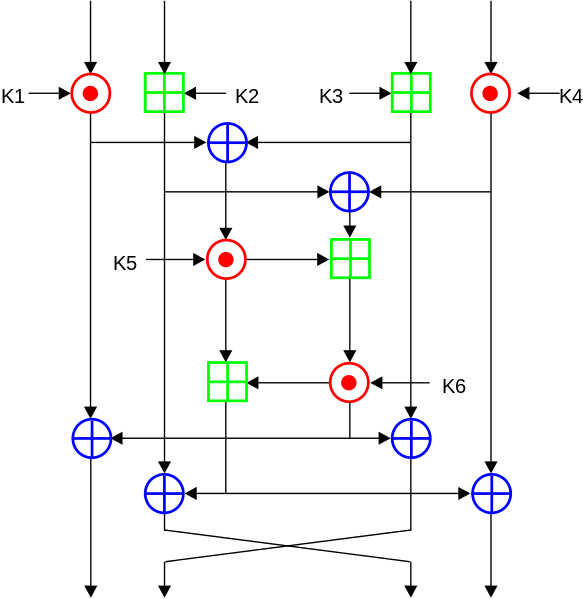
\includegraphics[width=0.4\linewidth]{img/fig_idea-step.png}
	\caption{Schéma šifrovacího kroku \cite{wiki.IDEA}}
	\label{fig:idea-step}
\end{figure}

Blok dat je rozdělen na čtyři části o velikosti 16b a zašifrován osmi iteracemi transformací znázorněných ve schématu znázorněném na Obrázku \ref{fig:idea-step}. Po aplikování iterací šifrovacího kroku je na jejich výstup použita výstupní transformace znázorněná Obrázkem \ref{fig:idea-half-step}.

\begin{figure}[h]
	\centering
	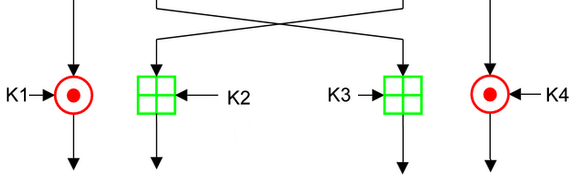
\includegraphics[width=0.4\linewidth]{img/fig_idea-half-step.png}
	\caption{Schéma výstupní transformace \cite{wiki.IDEA}}
	\label{fig:idea-half-step}
\end{figure}

Každá iterace používá různé pod-části klíče, které jsou odvozeny z původního 128b klíče bitovou rotací vlevo o 25 pozic. Tyto pod-části klíče jsou velké 16b, stejně jako části bloku dat šifrovacím procesu.
Iterace ifrovacího krok používají 6 podklíčů a výstupní transformace 4 podklíče, což je dohromady 52 podklíčů následujícím způsobem:
\begin{enumerate}
\item Hlavní klíč je rozdělen na 8 pod-částí, které jsou přímo použity.
\item Pokud nebylo vygenerování 52 podčástí, hlavní klíč je bitově cyklicky posunut vlevo o 25 pozic a pokračuje se od kroku 1.
\end{enumerate}


\subsection{Implementace řešení}
Aplikace je dělena do samostatných celků podle Principu Jedné Odpovědnosti. Hlavní částí je třída šifry, \texttt{IdeaCodec}, která dokáže metodami \texttt{encode} a \texttt{decode} zpracovat vstupní proud a zpracovaná data uložit na výstupní proud.

Samotné šifrování potom probíhá pomocí tříd \texttt{IdeaStep} a \texttt{IdeaHalfStep}, které obsahují samotné aritmetické operace šifrování. Každý krok nese informaci o datech na jeho vstupu a o prováděné operaci, tzn. šifrování nebo dešifrování.
Kroky dále umožňují přímé přesměrování šifrovaných dat do následujícího kroku anebo jejich získání pro další použití.

O správnost velikosti a formát načítaných a ukládaných bloků dat se stará třída \texttt{IdeaDataChannel}, která zapouzdřuje vstupní a výstupní proud.

Parametr třídy šifry je klíč, \texttt{IdeaKey}, tedy třída která z generického kryptografického klíče vygeneruje šifrovací a dešifrovací klíče. Generickým klíčem se rozumí třída \texttt{CryptoKey}, která je tvořena polem bytů.
Aplikace obsahuje konkrétní implementaci generického klíče \texttt{HexDecKey}, která umožňuje zpracování hexadecimálních znaků do požadované délky. Při poskytnutí více bytů, než kolik bytů odpovídá požadované délce, jsou nadbytečné znaky XORovány již existující částí klíče.

Aplikace je dostatečně dekomponována pro možné oddělení samotné výkonné logiky a jejího spouštění a obsahuje příkazové rozhraní pro zpracovávání vstupů z příkazové řádky.

\section{Uživatelská dokumentace}
Aplikaci je možné spouštět spuštěním příkazu:\\
{\centering \texttt{ java -jar kiwi-idea.jar <operace> <klíč> <vstup> <výstup> [-s]}}
Významy parametrů jsou:
\begin{itemize}
	\item \textbf{operace} možné hodnoty jsou: "encode" nebo "decode"
	\item \textbf{klíč} řetězec hexadecimálních znaků o minimální délce 32 znaků (128b).
	\item \textbf{vstup} a \text{výstup} cesty k souborům vstupu a výstupu
	\item  \textbf{\lbrack-s\rbrack} tichý režim: aplikace nevypíše žádný výstup na standarní ani chybový výstup a pouze vrátí návratovou hodnotu
\end{itemize}

V případě nesprávně zadaných parametrů aplikace vypíše odpovídající chybové hlášení a zobrazí nápovědu pro spouštění se stručným popisem parametrů.

V bezchybném stavu aplikace po zašifrování zobrazí, kolik dat bylo celkem zpracováno a kolik času zadaná operace zabrala.

\section{Závěr}
Práce obsahuje implementaci šifry International Data Encryption Algorithm pro šifrování a dešifrování souborů. Správná funkcionalita jednotlivých částí je ověřena pomocí automatických testů frameworku JUnit 4 v rozsahu 100\% výkonné logiky šifry.
\bibliographystyle{abbrv}
{\raggedright\small
	\bibliography{literatura}
}

%------------------------------------------

\end{document}
